%%%%%%%%%%%%%%%%%%%%%%%%%%%%%%%%%%%%%%%%%%%%%%%%%%%%%%%%%%%%%%%%%%%%%%%%%%%%%%%%
%Objetivo: Descrever os principais conceitos relativos a Manutenção de Software
%		   envolvidos na dissertação
%Autores: Vagner Clementino <vagnercs@dcc.ufmg.br>
%		  Rodolfo Resende <rodolfo@dcc.ufmg.br>
%Criação: Ter Set 13 19:22:37 BRT 2016
%Modificação: qua fev 15 08:27:43 BRST 2017
%Revisão: dom fev 12 18:37:18 BRST 2017
%%%%%%%%%%%%%%%%%%%%%%%%%%%%%%%%%%%%%%%%%%%%%%%%%%%%%%%%%%%%%%%%%%%%%%%%%%%%%%%%

\chapter{Manutenção de Software: Uma Visão Geral}
\label{ch:visao-geral-manutencao}

Uma tendência natural do software é evoluir a fim de atender aos novos
requisitos e alterações do ambiente no qual ele está inserido. Em uma série de
estudos, Lehman propõe um conjunto de leis sobre a evolução do software. Dentre
elas podemos destacar as leis da Mudança Contínua (Continuing Change) e da
Complexidade Crescente (Increasing complexity). A primeira diz que um programa
que é utilizado em um ambiente real deve mudar ou se tornará progressivamente
menos útil~\cite{lehman1980understanding}. A lei da Complexidade Crescente
(Increasing complexity) afirma que quando um sistema em evolução muda, sua
estrutura tende a se tornar mais complexa. Nesta situação, recursos extras devem
ser disponibilizados a fim de preservar e simplificar a estrutura do
software~\cite{lehman1980understanding}. As leis de Lehman tem sido validadas,
especialmente aquelas relacionadas a tamanho e complexidade do software. Em um
trabalho sobre o tema Yu \& Mishra~\cite{{yu2013empirical}} examinaram de forma
empírica as Leis de Lehman em relação a evolução da qualidade do software. O
estudo demonstrou, tomando como base a métrica proposta, que a qualidade de um
produto de software declinará a menos que uma restruturação seja realizada.

Conforme exposto, a mudança em um produto de software é inevitável. Desta forma,
é importante a existência de uma área de estudo preocupada com o gerenciamento e
controle destas mudanças. Dentro do escopo da Engenharia de Software esta tarefa
fica a cargo da Manutenção de Software.  Nas próximas seções discutimos os
conceitos básicos que mostram onde e como a Manutenção se encaixa dentro da
Engenharia de Software. São apresentados os conceitos que fazem da Manutenção de
Software uma disciplina distinta.
\todobegin{Sugestão de apoiar os conceitos descrito com base em um livro ou
	artigo}
Os conceitos estão aderente com a literatura da área em especial com a ISO
\textit{14764:2006}, o \textit{Corpo de Conhecimento em Engenharia de
	Software}~\cite{4425813}, e o livro escrito por Tripathy \& Naik com foco
nos praticantes da manutenção de software~\cite{tripathy2014software}.
\todoend
%Percebida a importância do processo de manutenção de software, alguns trabalhos
%foram propostos visando mensurar o seu custo bem como propor processos com o
%objetivo de reduzir o esforço envolvido neste tipo de atividade.
%
%No trabalho de Herrin~\cite{Herrin:1985:SMC:323287.323383} foi proposto um
%modelo matemático com o objetivo de avaliar o impacto financeiro no orçamento
%de uma universidade devido às atividades de manutenção no sistema de
%processamento de dados da instituição. O modelo propõe que o valor disponível
%para desenvolvimento de um novo sistema é função inversa do custo de manutenção
%do software existente. Desta forma, o fato de se manter um sistema durante
%muito tempo poderá impossibilitar a aquisição ou mesmo o desenvolvimento de um
%novo.
%
%No estudo de Hirota et al.~\cite{hirota1994approach} é proposta a utilização da
%técnica Análise de Ripple para estimar o custo da manutenção de software. O
%termo ``efeito Ripple'' foi utilizado pela primeira vez em um artigo publicado
%por Haney~\cite{haney1972module} para descrever a forma que a mudança em um
%módulo poderia causar alterações em outras partes do
%sistema~\cite{bilal2005using}. A Análise Ripple é, portanto, uma técnica para
%analisar o fluxo de dados de variáveis dentro de um determinado programa. Os
%valores retornados pela aplicação do método são denominados Complexidade de
%Ripple. Os resultados demostraram que a Complexidade de Ripple está mais
%relacionada ao entendimento do software do que as métricas padrão, como linhas
%de código, complexidade ciclomática e pontos de função. Desta forma, a
%Complexidade de Ripple poderia ser utilizada, por exemplo, para predizer os
%custo de manutenção de um sistema, bem como a necessidade de substituição do
%mesmo.
%
%Mediante o uso de Redes Neurais Shula \& Misra
%\cite{Shukla:2008:ESM:1342211.1342232} propõe um estudo para medir o custo de
%manutenção de software. O trabalho discute a utilização de outras métricas além
%de linha de código e pontos de função para medir  tamanho e custo do processo
%de manutenção. Os resultados demonstraram a possibilidade de construir um
%modelo para medir o custo utilizando Redes Neurais. Contudo, os resultados são
%sensíveis a escolha da arquitetura e parâmetros de treino, os quais idealmente
%deveriam ser preparados por um especialista no sistema (oráculo).
%
%A dinamicidade do ambiente de negócios tem levado a diversas organizações a
%adotar as metodologias propostas pelos agilistas pelo fato delas auxiliarem no
%atendimento das exigências do cliente~\cite{Devulapally2015}. Esta tendência é
%mais forte no desenvolvimento de software e nos últimos anos vem ocorrendo de
%forma gradativa na manutenção.
%
%No trabalho de Kajko-Mattsson \& Nyfjord~\cite{4755767} foi proposto um modelo
%ágil para manutenção que apropria diferentes práticas do Extreme Programming e
%do Scrum. Segundo os autores a junção desta duas metodologias possibilita a
%inclusão de práticas úteis tanto do ponto de vista do gerente do projeto bem
%como dos desenvolvedores. O modelo encoraja diversas práticas tais como
%\textit{product backlog}, testes antes da codificação, planejamento iterativo,
%dentre outras.
%
%A adoção na manutenção de software de algumas práticas propostas pelos
%agilistas foram analisadas durante 08 meses em estudo realizado por Svensson \&
%Host~\cite{1402140}. Ao utilizar o Extreme Programming (XP) no processo de
%manutenção os autores concluíram que é muito difícil fazer uso do XP sem que
%sejam realizadas adequações no desenho de diversas práticas para desta forma
%adequar às necessidades do time de desenvolvimento.
%
%O estudo Heeager \& Rose~\cite{Heeager2015} propõe um conjunto de nove
%heurísticas com o objetivo de ajudar aos profissionais da manutenção de
%software na adoção de práticas propostas pelos agilistas. O trabalho consistiu
%da inclusão do Scrum na rotina de trabalho do departamento de manutenção de
%software de uma organização de grande porte. Os autores argumentam que os
%métodos ágeis, quando aplicado ao trabalho de desenvolvimento, têm certas
%características relativamente bem compreendidas, no entanto o trabalho de
%manutenção difere do de desenvolvimento em certos aspectos e, portanto, é
%desafiador a implementação de métodos ágeis em um departamento de manutenção.
%
\section{Conceitos Fundamentais}
\label{sec:conceitos_basicos}

Esta seção introduz os conceitos e terminologias que ajudam no entendimento do
papel e finalidade da Manutenção de Software. De uma maneira geral, podemos definir
atividade de manter software como a totalidade das ações necessárias para
fornecer suporte a um produto de software. Entretanto, encontramos na literatura
outras definições mais elaboradas sobre a área.

Manutenção de Software é definida pela IEEE 1219~\cite{ISO-1219-1998}-~Padrão para a
Manutenção de Software, como a modificação de um produto de software após a sua
entrega com o objetivo de corrigir falhas, melhorar o desempenho ou outros
atributos com a finalidade de adaptar o software às modificações ambientais. O
padrão cita a ocorrência de atividade de manutenção antes da entrega
propriamente dita, contudo, de forma concisa.

Posteriormente a IEEE/EIA 12207~-~Padrão para o Processo de Ciclo de Vida do
Software~\cite{ISOIEC-12207-2008}, retrata a manutenção como um dos principais
processos no ciclo de vida do software. Em seu texto a manutenção é vista como
atividade de modificação do código e da documentação associada e ocorre devido a
algum problema ou necessidade de
melhoria~\cite{IEEEComputerSociety:2014:GSE:2616205}.  Por outro lado a ISO/IEC
14764~-~Padrão para Manutenção de Software~\cite{1703974} enfatiza aspectos
iniciais do esforço de manutenção como, por exemplo, o planejamento.

De maneira relacionada, \textit{Manutenibilidade} é a propriedade de um sistema
ou componente de software em relação ao grau de \textit{facilidade} que ele pode
ser corrigido, melhorado ou adaptado~\cite{{159342}}. A
ISO/IEC~9126~-~01~\cite{ISOIEC9126} define a Manutenibilidade como uma
característica de qualidade do processo de Manutenção.

\todobegin{A frase: ``O conceito de evolução de software carece de uma definição
	padrão na literatura, contudo, pesquisadores e profissionais utilizam o
	termo como substituto preferido para manutenção'', foi removida.}

Apesar das diversas definições para Manutenção de Software é possível
identificar dois aspectos comuns: manter e evoluir. Embora exista o entendimento
que os processos de manutenção e evolução possuem características distintas, não
está nos objetivos desta dissertação discutir e apresentar tais diferenças. Neste
sentido, utilizamos os termos \textit{manter} e \textit{evoluir} software de
forma intercambiáveis.
\todoend

A Manutenção é necessária para garantir que o software seja capaz de satisfazer
os requisitos dos usuários. Neste sentido, a atividade de manter software pode
ser vista como um desenvolvimento contínuo, sobretudo, pelo fato que alguns
sistemas nunca estão completos e continuam a evoluir.

\section{Requisição de Mudança}
\label{sec:requisição_de_mudanca}

\subsection{Tipos de Requisições de Mudança}
\label{subsec:tipos_de_requisicoes_mudanca}

As manutenções em software podem ser divididas em \textit{Corretiva, Adaptativa,
	Perfectiva e Preventiva}~\cite{Lientz:1980:SMM:601062,159342}.  A Manutenção
Corretiva lida com a reparação de falhas encontradas. A Adaptativa tem o foco na
adequação do software devido à mudanças ocorridas no ambiente em que ele está
inserido. A Perfectiva trabalha para detectar e corrigir falhas latentes. A
Preventiva preocupa com atividades que possibilitem aumento da manutenibilidade
do sistema.  A ISO 14764~\cite{1703974} propõe a divisão da tarefa de
manutenção nos quatro tipos descritos anteriormente e propõe que exista um
elemento comum denominado Requisição de Mudança (RM) que representa as
características comuns a todas aqueles tipos de manutenção. A
Figura~\ref{fig:modification-request} exibe a classificação das RM's conforme
discutido pela ISO\@.

\begin{figure}[hbtp] \centering 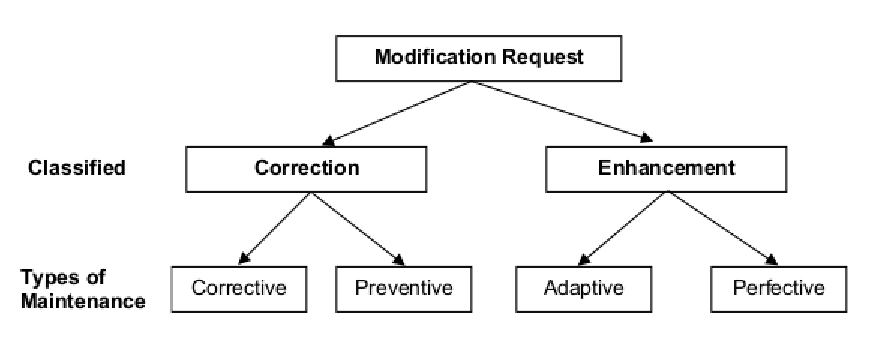
\includegraphics[width=.75\textwidth]
	{chapter-intro/img/modification_request.eps} \caption{Tipos de manutenção
		segundo a norma ISO/IEC 14764. Extraído de~\cite{1703974}}
\label{fig:modification-request} \end{figure}

A ISO/IEC 14764 classifica as manutenções adaptativas e perfectivas como
me\-lho\-ri\-as e agrupa as manutenções corretivas e preventivas em uma única
categoria de correção, conforme exibido na
Tabela~\ref{tab:categorias_requisicao_mudanca}. A manutenção preventiva é
frequentemente realizada em produtos de software onde atributos de segurança são
mais críticos.

\begin{table}[htpb] \centering 	\begin{tabular}{l|l|l|} \cline{2-3} &
		\textbf{Correção} & \textbf{Melhoria} \\ \hline
		\multicolumn{1}{|l|}{\textbf{Pró-ativa}} & Preventiva & Perfectiva \\
		\hline \multicolumn{1}{|l|}{\textbf{Reativa}} & Corretiva & Adaptativa
		\\ \hline \end{tabular}\caption{Categorias da Requisição de Mudanças.
		Adaptado de
		SWEBOK~\cite{4425813}}\label{tab:categorias_requisicao_mudanca}
\end{table}

Alguns pesquisadores e profissionais da manutenção entende que a manutenção
preventiva como um subconjunto da perfectiva~\cite{thipathy2014software}.
Segundo Tripathy \& Naik~\cite{tripathy2014software} uma Requisição de Mudança
(RM) é o veículo para registar as informações sobre o defeito, evolução ou
melhoria de um sistema. Em outras palavras, relatos de defeito ou requisições de
melhorias são documentadas como uma RM. A
Figura~\ref{fig:diagrama-classe-requisicao-mudancas} exibe um modelo conceitual
de uma RM no escopo desta dissertação.

\todobegin{Incluída uma imagem para representar que a Requisição de Mudanças
	representam um elemento comum de relatos de defeitos, evolução ou melhoria
	de um sistema} 
\begin{figure}[htpb]
	\centering
	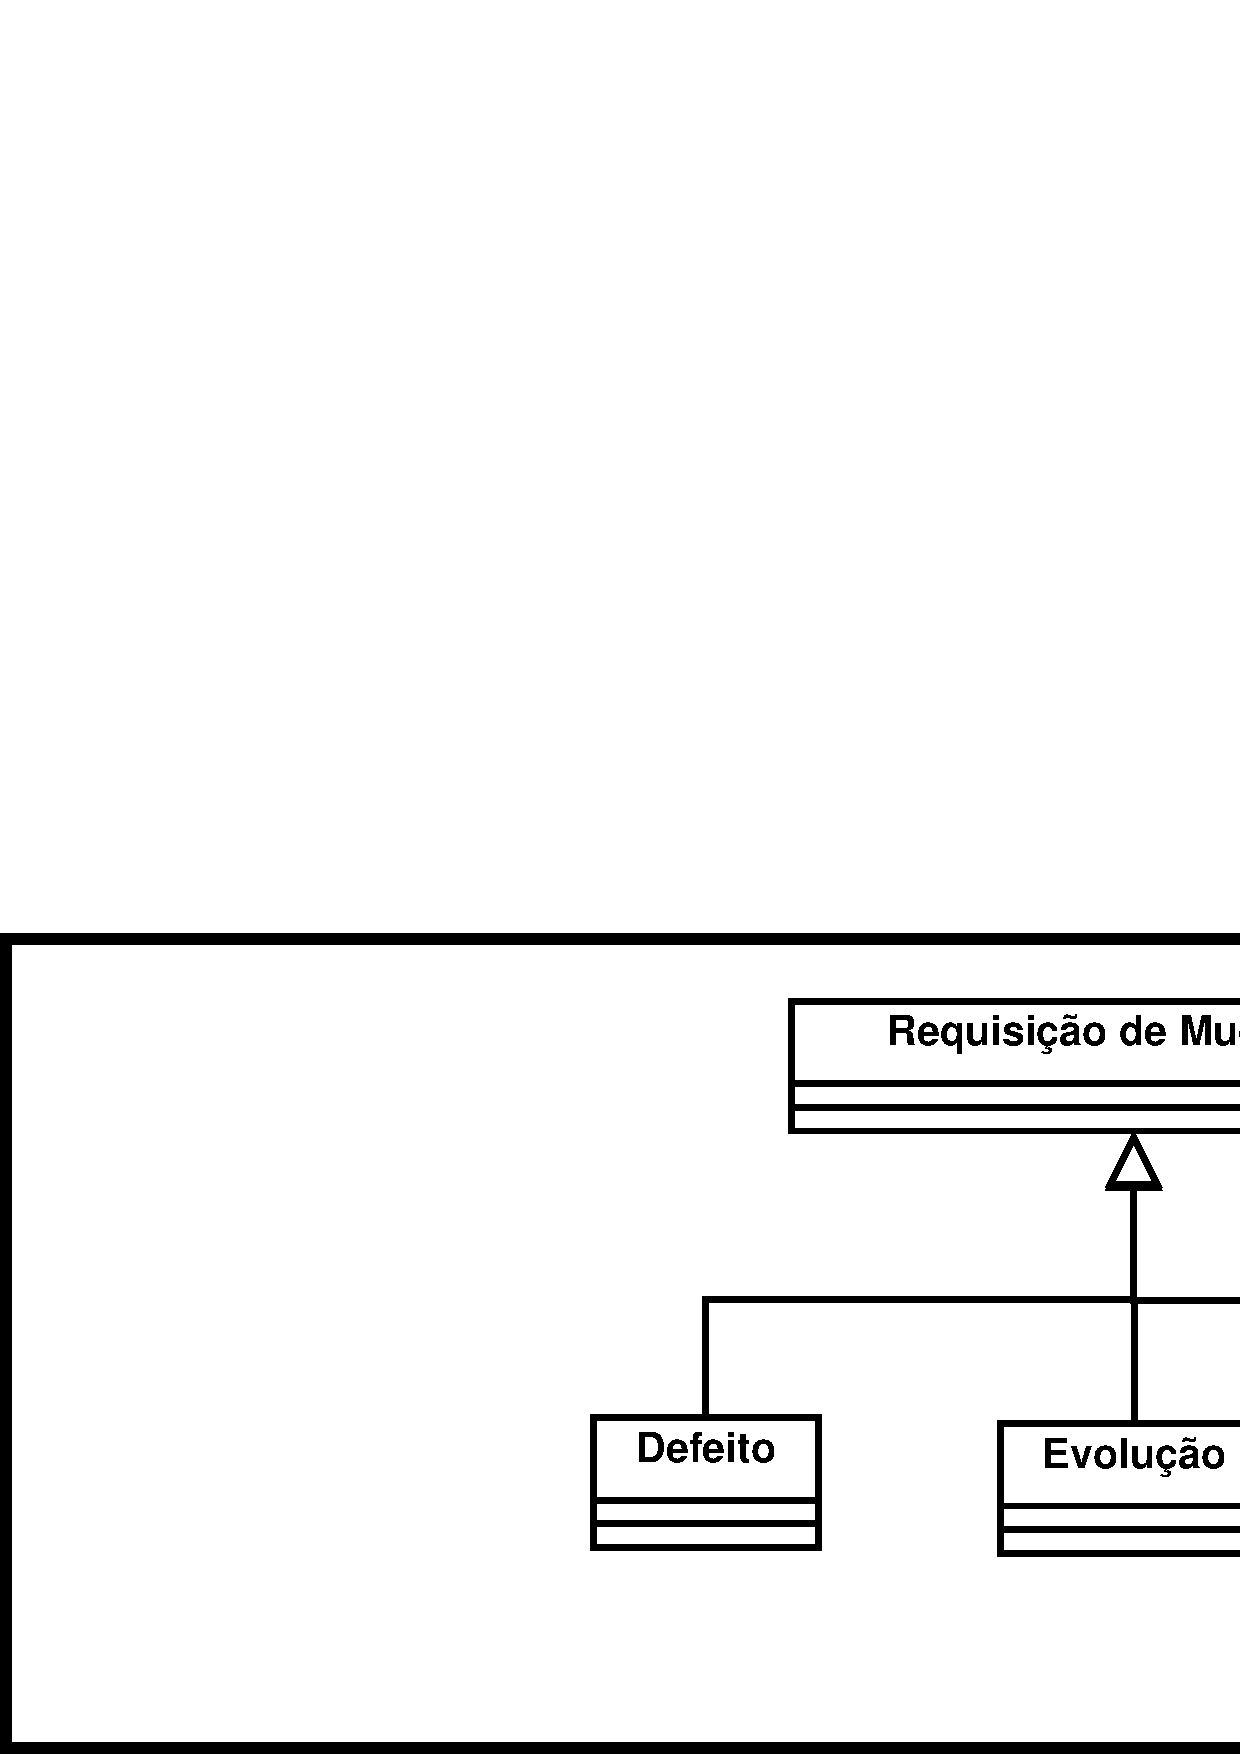
\includegraphics[width=0.8\linewidth]{./chapter-manutencao-software-visao-geral/img/diagrama-classe-conceitual-requisicao-mudancas.pdf}
	\caption{Modelo conceitual de uma Requisição de Mudanças}
	\label{fig:diagrama-classe-requisicao-mudancas}
\end{figure}
\todoend

As principais informações contidas em uma RM podem ser visualizadas no modelo
exibido na Figura~\ref{fig:diagrama-classe-atributos-requisicao-mudancas}. O
modelo é uma adaptação daquele proposto por Singh e outros~\cite{singh2011bug}
que reflete um processo genérico de relatar uma RM.

\begin{figure}[htpb]
	\centering
	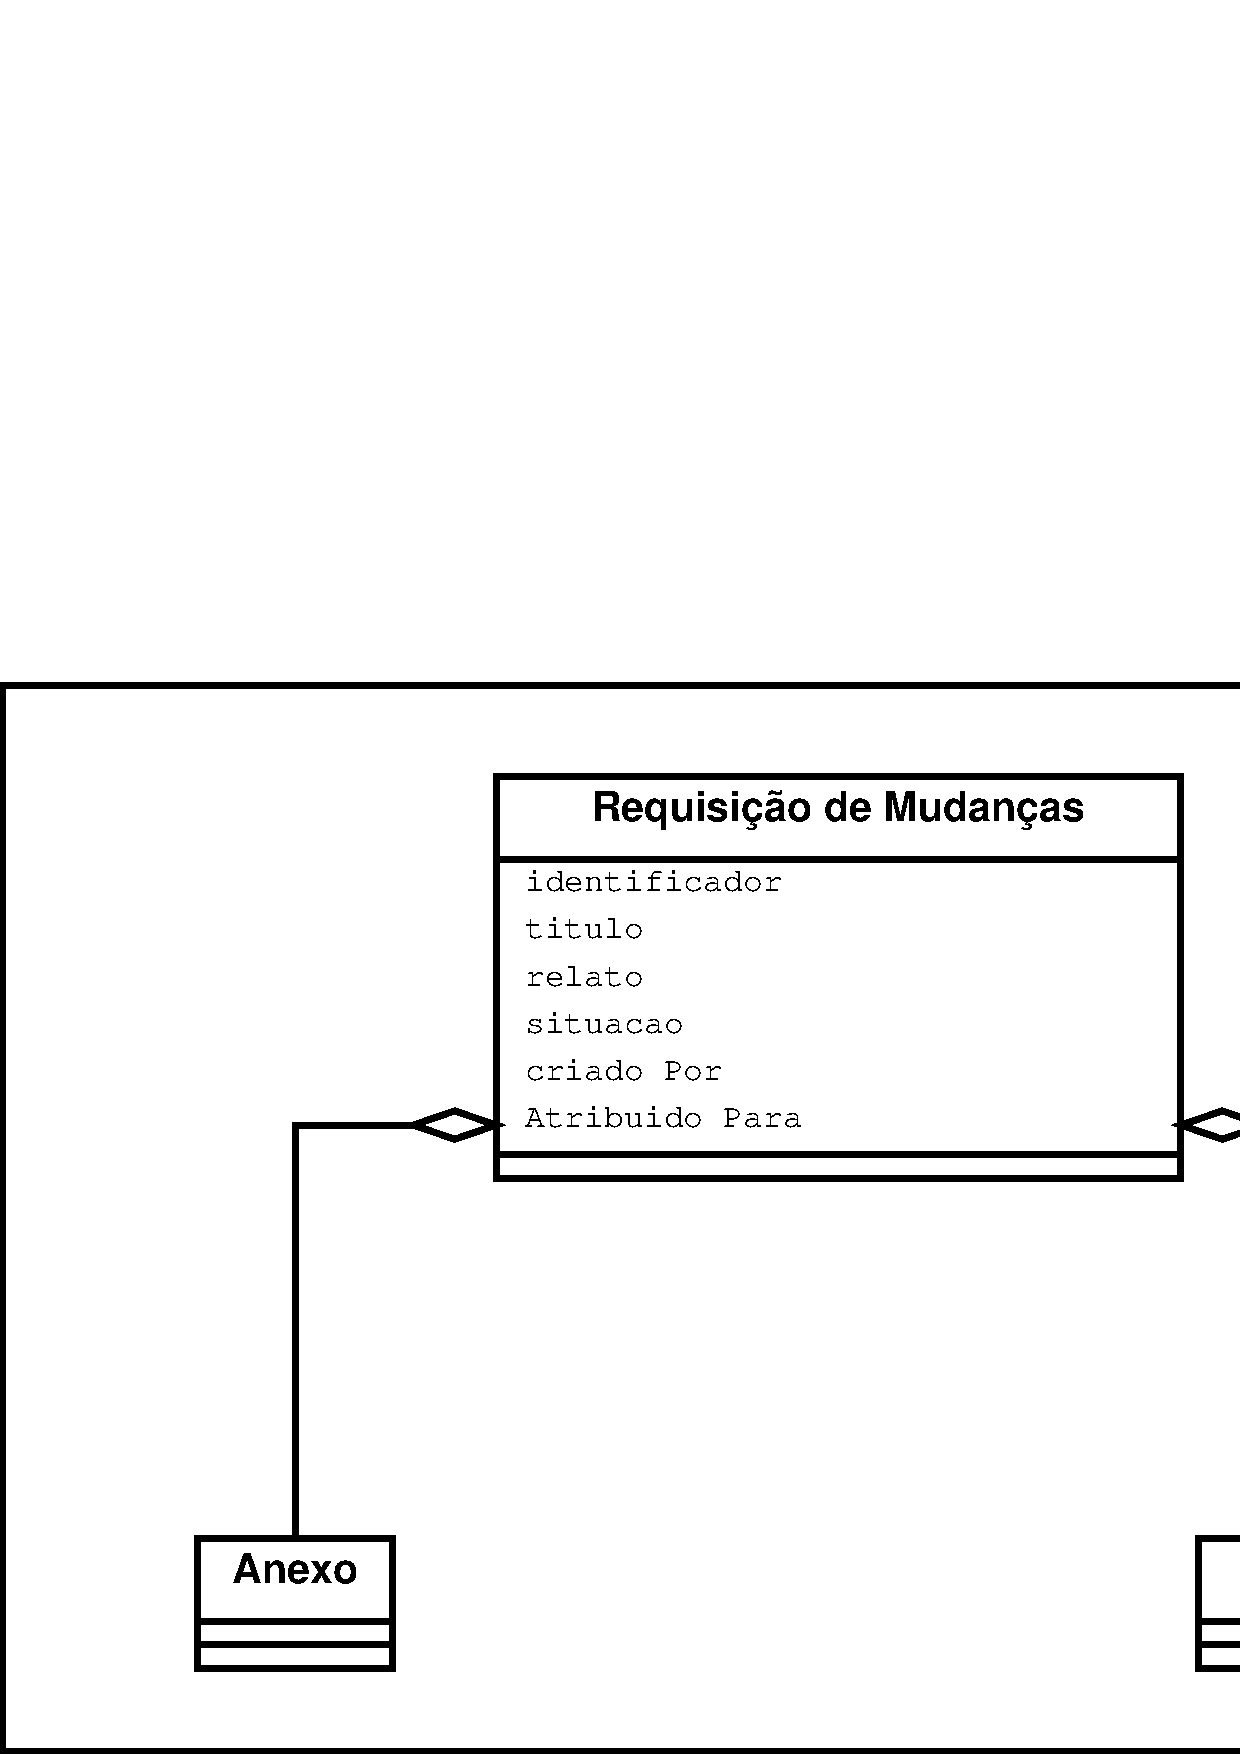
\includegraphics[width=0.8\linewidth]{./chapter-manutencao-software-visao-geral/img/diagrama-classe-atributos-requisicao-mudancas.pdf}
	\caption{Informações que compõem uma RM}
	\label{fig:diagrama-classe-atributos-requisicao-mudancas}
\end{figure}

Os principais conceitos envolvidos no modelo são listados  a seguir:.

\begin{description}
	\item [Identificador] Sequência de caracteres,  geralmente númerica,  que
		permite distinguir de maneira única uma RM.
	\item [Sumário] Um título ou resumo da RM.
	\item [Relato] Descrição detalhada da RM incluindo o que, onde, por que,
		como e quando a RM ocorreu. A mensagem que aparece durante a operação do
		sistema pode ser incluída, bem como a entrada inserida e a saída
		esperada.
	\item [Situação] A situação atual de uma RM\@. Representa os diversos estados
		que uma RM possui em seu ciclo de vida.
	\item [Criado Por] Nome da pessoa ou um identificador  já registrado no
		sistema de quem está relatando a RM\@.
	\item [Atribuido Para] A RM pode ser atribuída a uma pessoa específica caso
		ELA seja capaz de resolvê-la, caso contrário, a RM será atribuída para
		alguém que possui o papel de agendador.
	\item [Anexo] Refere-se a informações não textuais que podem ser incluídos
		na RM como casos de teste, capturas de tela com o defeito apresentado
		pelo sistema ou cadeia de registros de ativação (stack trace).
	\item [Comentário] Registra o histórico de discussões realizadas durante o
		processo de resolução da RM\@.
\end{description}

Em alguns textos sobre manutenção de software o relato, apesar de ser um
atributo de uma RM, é utilizado como sinônimo da mesma. Em outros contextos, as
informações contidas em determinada RM pode mudar. Tais campos, denominados de
pré-definidos, no relatório de bugs fornecem uma variedade de metadados
descritivos tais como \textit{importância, prioridade, gravidade, componente, e
	produto}~\cite{zhang2016literature}. A Figura~\ref{fig:rm-exemplo} exibe um
exemplo representativo de uma RM contendo todos os elementos básicos descritos
no modelo, tais como identificador, sumário, relato, dentre outros.

\begin{figure}[htpb]
	\centering
	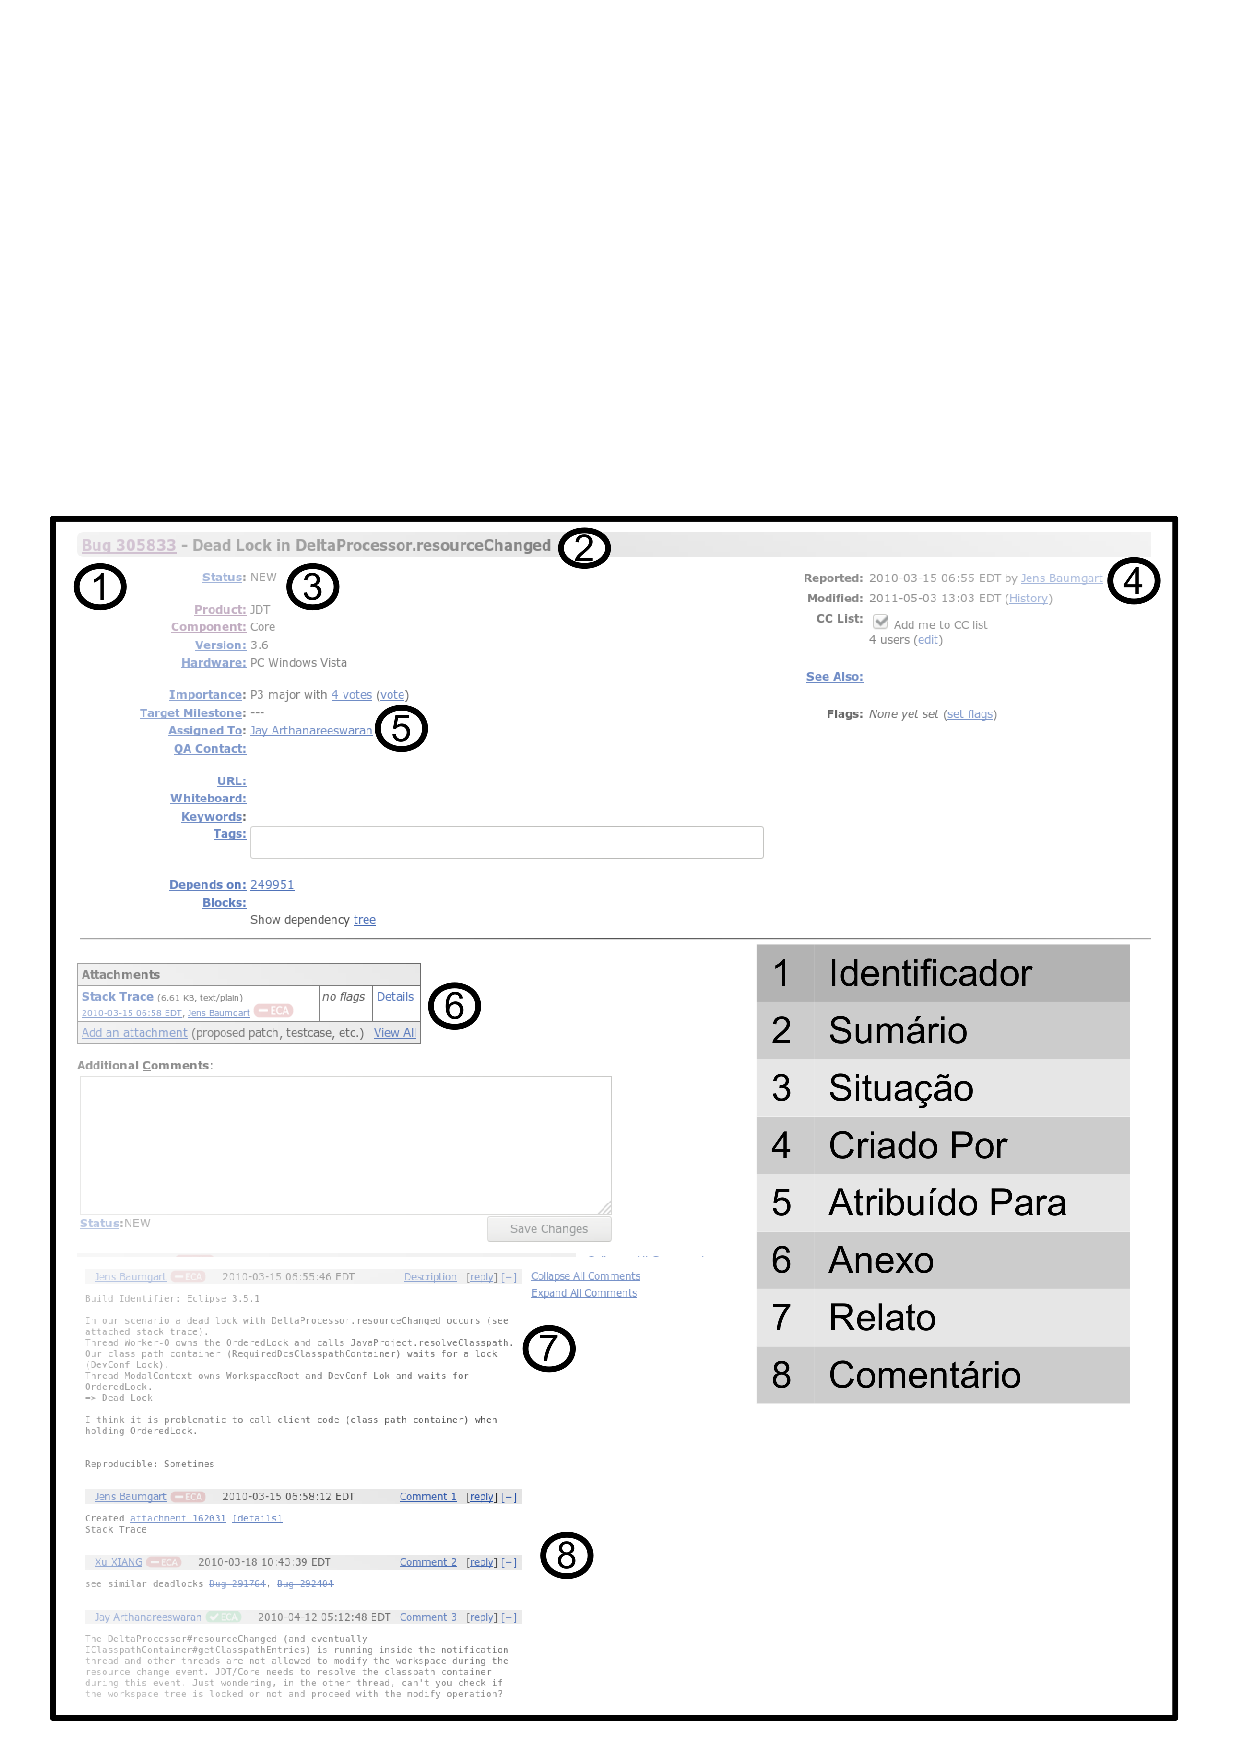
\includegraphics[width=0.8\linewidth]{./chapter-manutencao-software-visao-geral/img/rm-exemplo.pdf}
	\caption{Um exemplo de uma RM do Projeto Eclipse}
	\label{fig:rm-exemplo}
\end{figure}

Em síntese, apesar das diferentes nomenclaturas existentes na literatura
(demanda, bug, defeito, bilhete, tíquete, requisição de modificação, relato de
problema) uma Requisição de Mudança representa o relato, independente de sua
estrutura, que visa gerar a manutenção ou evolução do software. Nesta
dissertação estas diferentes nomenclaturas serão utilizados de forma
intercambiáveis.


\subsection{Ciclo de Vida de uma Requisição de Mudança}
\label{sub:fluxo_de_trabalho_requisicao_mudanca}
\todobegin{Incluída uma discussão sobre os diversos ``estados'' que um determinada RM pode ter. Os conceitos foram apoiados no livro Software
	Evolution and Maintenance de Priyadarshi e Kshirasagar}

Uma RM descreve os desejos e
necessidades dos usuário que os sistema é esperado implementar. Durante o
processo de relatar uma RM, dois fatores devem ser levados em
conta~\cite{tripathy2014software}:

\begin{itemize}
	\item \textit{Corretude da RM:} uma RM deve ser descrita de forma não ambígua tal
		que seja fácil revisá-la afim de determinar sua corretude. O
		``formulário'', como por exemplo os campos a serem preenchidos em uma
		FGRM (vide
		Seção~\ref{sec:ferramentas_de_gerenciamento_requisicoes_de_mudanca})
		quando uma RM é criada, é a chave para efetiva interação entre a
		organização que desenvolver o software e os seus usuários. O formulário,
		neste sentido, documenta informações essenciais sobre mudanças no
		software, hardware e documentação.
   \item \textit{Comunicação clara das RM's com as partes
		   interessadas:\footnote{Na
			   Seção~\ref{subsec:man_visao_geral_papeis_na_manutencao_de_software}
			   discutiremos em maior detalhe as diferentes partes interessadas
			   no contexto da manutenção de software.}} as RM'S necessitam ser
	   claramente comunicadas para as parte as interessadas, incluindo os
	   mantenedores, tal que elas não sejam interpretadas de forma distintas. O
	   resultado de avaliar de maneira distinta uma RM pode ser contra-produtivo:
	   \textit{(i)} A equipe que realiza mudanças no sistema e a equipe que
	   executa testes podem ter  visões contraditórias sobre a qualidade do
	   software; \textit{(ii)} O sistema alterado pode não atender às
	   necessidades e desejos dos usuários finais.
\end{itemize}

Uma RM deve ser representada de uma forma não ambígua e estar disponível de
maneira centralizada. No caminho entre o usuário e os desenvolvedores uma RM
pode estar em diferentes estágios. O ciclo de vida de uma RM pode ser ilustrado
como diagrama de estados conforme ilustrado na
Figura~\ref{fig:diagrama-estado-rm}.

\begin{figure}[htpb]
	\centering
	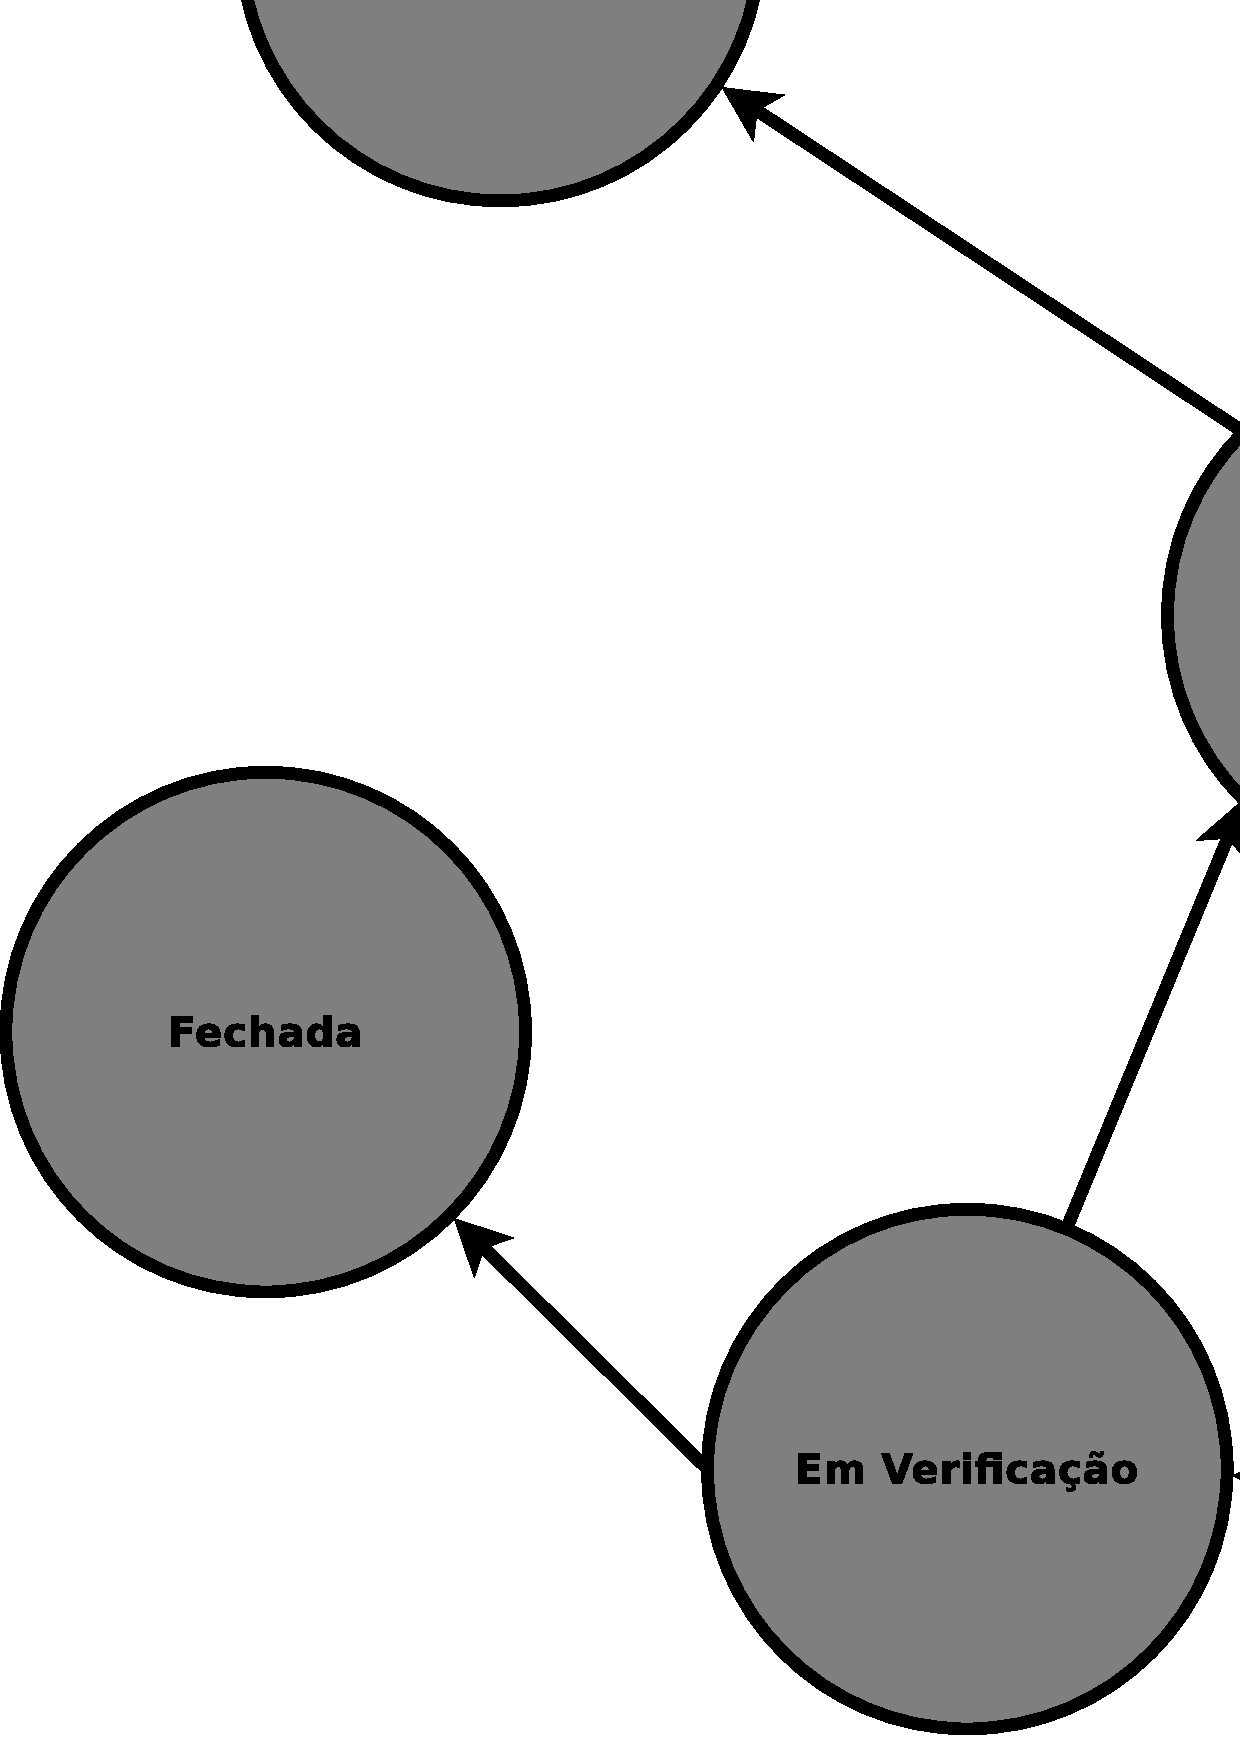
\includegraphics[width=0.8\linewidth]{./chapter-manutencao-software-visao-geral/img/diagrama-estado-rm.pdf}
	\caption{Diagrama de estados de uma RM\@. Extraído
		de~\cite{tripathy2014software}}
\label{fig:diagrama-estado-rm}
\end{figure}

O modelo mostra a evolução de uma RM mediante os seguintes estados':
\textit{Submetida (Submit), Em Revisão (Review), Em análise (Analysis), Commit
	(Comprometida), Implementada (Implement), Em Verificação (Verification) e
	Fechada (Closed)}~\cite{tripathy2014software}. Uma determinada RM também
pode ser recusada o que a leva para o estado de mesmo nome (\textit{Decline}).
Por diversas razões a situação de uma RM para \textit{Recusada} a partir dos
outros estados. Por exemplo, o usuário conclui que modificações descritas na RM
não fazem mais sentido. A seguir apresentamos as características de cada um dos
estados que compõem o ciclo de vida de uma RM\@. Para cada estado pode haver um
mais papel que são responsáveis pela ações que são executadas. Uma discussão
sobre este papeis pode ser encontrada na
Subseção~\ref{subsec:man_visao_geral_papeis_na_manutencao_de_software}.

\paragraph{Submetida (Submit).}
\label{par:submetida)}

Este é estado inicial de uma RM recentemente envida. Geralmente, são os usuários
do sistema a fonte primária deste tipo de RM. Com base no nível de prioridade de
uma RM, ela é movida de \textit{Submetida} para \textit{Em Revisão}. Normalmente
\textit{Gerente de Requisição de Mudança} assume a responsabilidade desta
manipulação inicial das RM's e ele torna-se o ``dono'' da RM.

\paragraph{Em Revisão (Review).}
\label{par:em_revisao}
Normalmente, cabe ao \textit{Gerente de Requisição de Mudanças} manipulas as
RM's no estado \textit{Em Revisão} através das seguintes atividades:

\begin{itemize}
	\item Verificar se a RM submetida recentemente é uma duplicação de outra já
		existente. Se a RM é identificada como duplicada o estado da mesma é
		alterado para \textit{Recusada} normalmente com uma breve explicação e
		algum tipo de ligação para a RM original.
	\item Aceitar o nível de prioridade atribuído para a RM ou alterá-lo.
	\item Determinar o nível de severidade da RM: normal ou crítico.
	\item Caso por alguma razão as análises descritas anteriormente não possam
		ser realizadas, a RM é movida para o estado em \textit{Em análise}.
\end{itemize}

\paragraph{Em Análise (Analysis).}
\label{par:em_analise}
Neste estágio uma análise de impacto é conduzida para entender a RM e estimar o
tempo necessário para implementá-la. Após esta análise, caso se decida que não é
possível ou desejável atender a RM, então \textit{Rejeita} se torna o próximo
estágio da RM. Caso contrário a RM é movida para estado \textit{Commit} no qual
um desenvolver é atribuído como o  novo ``dono'' da RM. No caso do estado
\textit{Em Análise} o ``dono'' da RM é denominado \textit{Agendador}.

\paragraph{Comprometida (Commit).}
\label{par:commit}

A RM continua ``parada" no estado \textit{Comprometida} antes que as
modificações solicitadas estejam disponíveis em uma próxima versão do produto.
Neste estado a RM está a cargo do \textit{Gerente de Requisição de Mudança}.
Todas as RM's em que se tenha interesse em estar em uma versão específica do
software são revisadas. Algumas RM's podem ser incluídas em futuras versões do
sistema após acordo com as demais partes interessadas. Após
\textit{Comprometida} com determinado lançamento, a RM é movida para o estado
\textit{Em Implementação} para que o respectivo desenvolvimento e testes sejam
realizados.

\paragraph{Em Implementação (Implement).}
\label{par:em_implementacao}

No estágio de \textit{Em Implementação} diferentes cenários podem ocorrer:

\begin{itemize}
	\item A RM pode ser rejeitada caso sua implementação não seja factível.
	\item Caso a RM seja possível de implementar os desenvolvedores realizam a
		codificação e os testes unitários. A RM é movida de \textit{Em
			Implementação} para \textit{Em verificação}
\end{itemize}

\paragraph{Em Verificação (Verification).}
\label{par:em_verificacao}

No estão de verificação as atividades são controladas pela equipe de testes.
Para atribuir um veredito, a verificação pode ser realizada por um ou mais
métodos: demostração, análise, inspeção ou teste. Caso a verificação seja
realizada mediantes teste, então o software é executado com um conjunto de
teste. A inspeção significa revisar o código em busca de defeitos. A análise é
implica em demonstrar que o sistema está em operação. A situação da verificação
é fornecida em termos do grau de conformidade da RM: não conforme, parcialmente
conforme e completamente conforme. Caso nenhum método de teste é utilizada,
então uma nota explicando os detalhes da demostração, inspeção ou analise
realizada.

\paragraph{Fechada (Closed).}
\label{par:fechada}

Após a verificação de que a RM foi incorporada com sucesso ao software, a RM é
movida de \textit{Em verificação} para o estado \textit{Fechada}. Esta ação é
realizada pelo \textit{Analista de Qualidade} que o proprietário da RM durante o
estado de \textit{Em Verificação}.

\paragraph{Rejeitada (Decline).}
\label{par:rejeitada}
Conforme discutido uma RM pode ser rejeitada. Nestas situações a RM é movida
para um estado de mesmo nome. Dentre os diversos motivos que levam uma RM deixar
de ser feita podemos destacar: a RM deixar de produzir relevante impacto no
sistema; não é possível tecnicamente realizar o que foi solicitado na RM; a
equipe de qualidade conclui que as mudanças realizadas no software pela RM não
podem ser satisfatoriamente verificadas.
\todoend

\todobegin{Incluída a visão do processo de ciclo de vida de uma RM em projetos
	de código aberto.}
O modelo de ciclo de vida proposto por possui um foco na industria de software,
especialmente em organizações que possuem uma exclusivamente dedicada à
manutenção de software. Em outros contextos, como por exemplo em projetos de
software de código aberto, o processo de modificação dos estados de uma RM é um
pouco diferente.

No trabalho de Ihara e outros~\ref{ihara2009analysis}, foi conduzido um estudo
de caso nos projetos de código aberto Firefox e Apache em que um dos resultados
foi um digrama de estados que representa o processo de modificação de uma RM
utilizando uma FGRM. Este diagrama é representado na
Figura~\ref{fig:diagrama-estado-rm-codigo-aberto}.

\begin{figure}[htpb]
	\centering
	\includegraphics[width=0.8\linewidth]{./chapter-manutencao-software-visao-geral/img/diagrama-estado-rm-codigo-aberto.pdf}
	\caption{Um processo de modificação de uma RM utilizando uma FGRM. Adaptado
	de~\cite{ihara2009analysis}}
	\label{fig:diagrama-estado-rm-codigo-aberto}
\end{figure}

Os autores ponderam que apesar do processo de modificação de uma RM pode alterar
levemente de uma FGRM para outra, o diagrama apresentado na
Figura~\ref{diagrama-estado-rm-codigo-aberto} é capaz de representar de forma
substancial o processo de transição de uma RM. O processo é composto de três
diferentes fase: \textit{não tratada (untreated) , modificação (modification) e
verificação (verification)}.

A fase \textit{não tratada} foca em um subprocesso onde as RM's são relatadas em
uma FGRM, todavia não foi aceito ou atribuído a ninguém. A fase de
\textit{modificação} é um subprocesso onde as RM's são efetivamente modificadas.
Nesta fase uma RM é aceita e posteriormente atribuída a algum desenvolvedor.  A
fase de \textit{verificação} é o subprocesso membros com a responsabilidade de
garantia da qualidade verifica quais RM's modificadas foram corretamente
resolvidas. Caso uma RM modificada por um desenvolver não seja verificada, ela
poderia não ser reconhecida como finalizada (closed).

É possível acoplar o modelo proposto por Tripathy \&
Naik~\cite{tripathy2014software} naquele descrito por Ihara e
outros~\ref{ihara2009analysis}, especialmente por conta do segundo ser mais
genérico.  Neste dissertação utilizamos de forma geral o modelo contido no
trabalho de Ihara e outros. Nos casos em que houver necessidade de um maior
detalhamento do ciclo de vida de uma RM, a discussão tomara como base o modelo
de Tripathy \& Naik.
\todoend

\section{O processo de Manutenção de Software}
\label{sec:o_processo_de_manutecao_de_software}

\todobegin{Incluída localização da definição do texto tendo em vista que a
	referência possui mais de 400 páginas}
Em um relatório técnico~\cite{paulk1993key}, que descreve as principais práticas
que correspondem a cada nível de maturidade de um modelo de maturidade,
verificamos em seu glossário a seguinte definição de Processo de Software: é o
conjunto de atividades, métodos, práticas e transformações utilizadas para
desenvolvê-lo ou mantê-lo bem como seus artefatos
associados~\cite{paulk1993key}. Independente do contexto em que a manutenção
ocorra é importante que o processo esteja bem definido. Existe na literatura a
proposição de alguns modelos do processo de manutenção de software,
especialmente baseados em uma visão tradicional no qual desenvolvimento e
manutenção possuem uma clara separação. Recentemente os métodos propostos pelos
agilistas vêm sendo utilizados para manter software.  Esta tendência surge da
demanda crescente por serviços de manutenção com um retorno mais rápido para o
usuário.
\todoend

Nas próximas seções apresentamos alguns modelos encontrados na literatura na
perspectiva tradicional, ao mesmo tempo descrevemos propostas do uso da
metodologia dos agilistas na manutenção de software.

\subsection{Manutenção de Software Tradicional}
\label{subsec:manutenção_de_software_tradicional}

Em resumo, um processo de manutenção de software descreve as atividades e suas
respectivas entradas e saídas. Alguns modelos são descritos nos padrões IEEE
1219 e ISO/IEC 14764. O processo especificado no Padrão para Manutenção de
Software (IEEE~-~1219) indica que as atividades de manutenção de software iniciem
após a entrega do produto de software. O padrão também discute aspectos de
planejamento da manutenção. As atividades que compõe o processo são apresentas
na Figura~\ref{fig:ieee-1219-processo-man-software}.

\begin{figure}[htpb] \centering
	\includegraphics[width=0.7\linewidth]
	{chapter-manutencao-software-visao-geral/img/ieee-1219-98-processo-manutencao.png}
	\caption{IEEE 1219 -~Processo de Manutenção de Software}\label{fig:ieee-1219-processo-man-software}
\end{figure}

De maneira relacionada, na ISO/IEC 14764 as atividades que compõe o processo são
similares aquelas propostas na IEEE-~1219, exceto pelo fato que elas são
agregadas de uma forma diferente. O processo descrito na ISO/IEC~14764 são
exibidas na Figura~\ref{fig:ieee-14764-processo-manutencao}

\begin{figure}[htpb] \centering
	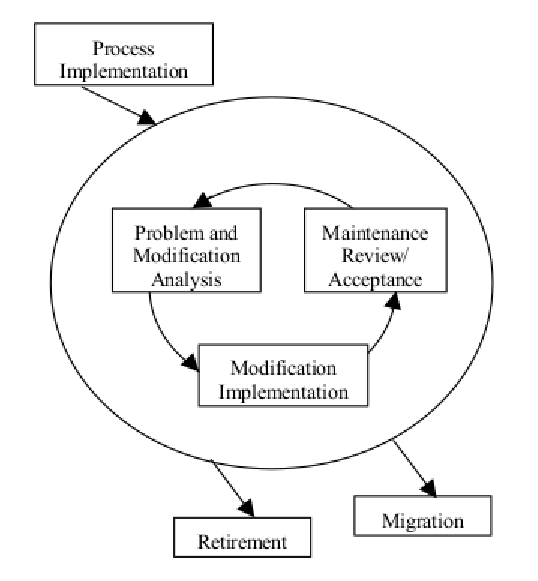
\includegraphics[width=0.7\linewidth]
{chapter-manutencao-software-visao-geral/img/ieee-14764-processo-manutencao.pdf}
	\caption{ISO/IEC~14764 Processo de Manutenção de Software}
\label{fig:ieee-14764-processo-manutencao} \end{figure}

As atividades de manutenção propostas na ISO/IEC 14764 são detalhadas em tarefas
conforme apresentadas a seguir:

\begin{itemize}
   	\item Implementação do Processo
   	\item Análise e Modificação do
		Problema
	\item Aceitação e Revisão da Manutenção
   	\item Migração
   	\item Aposentadoria do Software
\end{itemize}

É possível notar que algumas atividades realizadas durante a manutenção de
software são similares à outras presentes no desenvolvimento de software, como
por exemplo, análise de desempenho, codificação, teste e documentação. Outra
atividade comum à manter e desenvolver software é o gerenciamento dos
requisitos. Nas duas situações os profissionais responsáveis por controlar os
requisitos devem atualizar a do\-cu\-men\-ta\-ção  por conta de alterações
ocorridas no código fonte. Por outro lado certas atividades estão vinculadas
apenas ao contexto da manutenção de software. O Corpo de Conhecimento em
Engenharia de Software~\cite{4425813} destaca algumas delas:

\todobegin{Faltava referência sobre as atividades que seriam únicas ao processo
	de manutenção. Havida duvidas sobre se as atividades: Suporte ao Usuário,
	Suporte ao Uso de Software e Acordo de Nível de Serviço}
\begin{description}
	\item[Compreensão do programa:] atividades necessárias para obter um
		conhecimento geral do que um produto de software faz e como as partes
		funcionam em conjunto;
	\item[Transição:] uma sequência controlada e coordenada de atividades onde o
		software é transferido progressivamente do desenvolvedor para o
		mantenedor;
	\item[Aceitação/rejeição de Requisições de Mudança:] as modificações
		que ultrapassem determinado limiar de tamanho, esforço ou complexidade
		podem ser rejeitadas pelos mantenedores e redirecionadas para um
		desenvolvedor;
	\item[Suporte ao usuário:] uma função de suporte para o usuário final que
		aciona a avaliação, priorização ou avaliação de esforço das Requisições
		de Mudança;
	\item[Análise de impacto:] uma técnica para identificar áreas afetadas por
		uma potencial mudança;
	\item[Contratos de Acordo de Nível de Serviço (Service Level Agreements
		\@-\@ SLA):] acordos contratuais que descrevem os serviços e objetivos
		de qualidade.
\end{description}
\todoend

\subsection{Manutenção de Software na Perspectiva dos Agilistas}
\label{sub:manutenção_de_software_com_método_dos_agilistas}

Grande parte da literatura em Manutenção de Software trata de técnicas e
metodologias tradicionais da Engenharia de Software. Todavia, verifica-se uma
tendência que os departamentos dedicados à manutenção de software se mostrem
interessados nas metodologias dos agilistas e que tenham vontade de
experimentá-las em suas atividades~\cite{Heeager2015}.

No momento da elaboração desta dissertação boa parte dos textos em Engenharia de
Software tratarem desenvolvimento e manutenção como atividades com natureza
distintas, esta última pode adaptar características da primeira visando a
melhoria do seu desempenho. Dentre as práticas propostas pelos agilistas
passíveis de serem utilizadas em tarefas de manutenção é possível citar o
desenvolvimento iterativo, maior envolvimento do cliente, comunicação face a
face, testes frequentes, dentre outras.

Alguns resultados demonstram certa dificuldade para implantação da metodologia
dos agilista na manutenção de software~\cite{1402140}. Um dos possíveis
problemas é a necessidade de adequação das práticas da organização de modo que a
se adequar as necessidades do time de desenvolvimento.  Estudos apresentam
resultados relativos à melhorias no aprendizado e produtividade da equipe
mediante o aumento da moral, encorajamento e confiança entre os desenvolvedores,
o que propicia uma alta motivação durante o processo de manutenção de
software~\cite{Choudhari:2014:EIM:2557833.2557845}.

\todobegin{Conforme sugerido vou ``deslocada'' a discussão sobre os papéis
	dentro da manutenção de software. O testo foi revisado e para deixar mais
	claro foi utilizada diagrama de caso de uso.}

\subsection{Papéis na Manutenção de Software}
\label{subsec:man_visao_geral_papeis_na_manutencao_de_software}

As ações que alteram o estado de uma RM são realizadas por diversas pessoas
envolvidas no processo de manutenção de software que desempenham diversos
papéis. Os nomes e as atividades desenvolvidas por cada papel poderia variar de
um projeto para outro, contudo, é possível determinar uma classificação que
agrega um pouco comum deste diferentes papéis. Nesta dissertação, utilizamos a
classificação proposta por Polo e outros~\cite{Polo1999} cujo objetivo é definir
uma estrutura da equipe de manutenção de software mediante a clara identificação
das tarefas que cada membro deve executar. Os papéis propostos no estudo é
produto da aplicação da metodologia MANTEMA~\cite{756695} para manutenção em
projetos de software bancários espanhóis, em especial aqueles em que a área de
manutenção foi terceirizada (outsourcing). Os autores reforçam que apesar da
taxonomia de papéis ter sido criada em um contexto específico, ela pode ser
adequada para aplicação em outras situações.

No escopo deste trabalho removemos os papéis que segundo o nosso entendimento
estão mais vinculados a um contexto de manutenção terceirizada (outsourcing).
Além disso, dividimos o papel ``time de manutenção' (maintenance team) em
\textit{Desenvolvedor e Analista de Qualidade} por entendermos que são papéis
comuns a muito dos processos de manutenção existentes. Os papéis que compõe a
taxonomia proposta estão descritos a seguir:

\paragraph{Usuário Afetado:}
Indivíduo que utiliza o sistema ou sistemas que correspondente à RM que será
relatada. O defeito, a melhoria ou evolução no software, representada pela RM,
estão relacionadas com os desejos e necessidades deste papel.

\paragraph{Reportador:}
Responsável por registrar a Requisição de Mudança na FGRM\@. Geralmente,
qualquer pessoa envolvida no processo de manutenção de software pode relatar uma
RM. Neste sentido, as atividades relacionadas com o papel de Reportador podem
estar vinculados aos demais contidas nesta classificação. A
Figura~\ref{fig:diagrama-caso-uso-reportador} apresenta esta situação através de
um diagrama de caso de uso.

\begin{figure}[htpb]
	\centering
	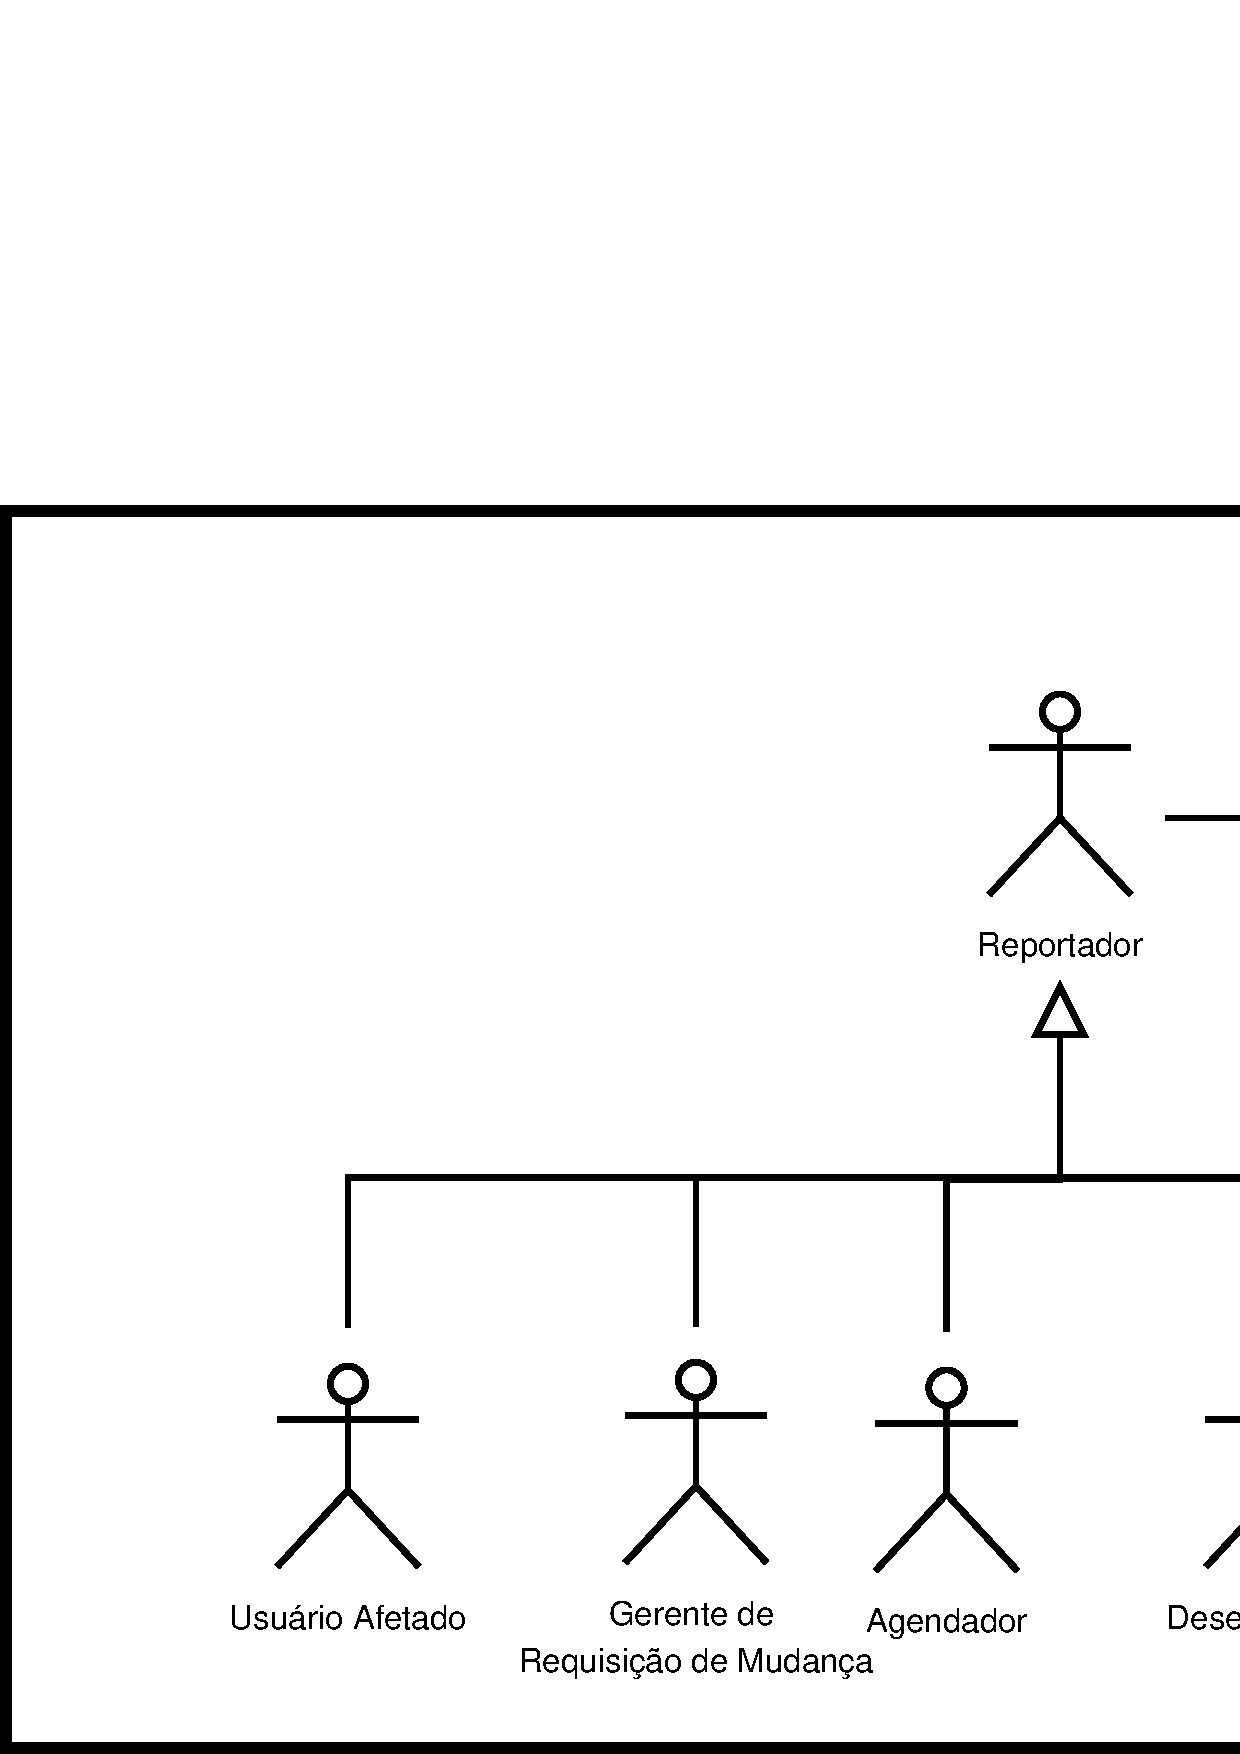
\includegraphics[width=0.8\linewidth]{./chapter-manutencao-software-visao-geral/img/diagrama-caso-uso-reportador.pdf}
	\caption{Diagrama de caso de uso do papel Reportador}
	\label{fig:diagrama-caso-uso-reportador}
\end{figure}

\paragraph{Gerente de Requisição de Mudança (Maintenance-request manager):}
Res\-pon\-sá\-vel por decidir se uma Requisição de Mudança será aceita ou
rejeitada e qual tipo de manutenção deverá ser aplicada. Posteriormente cabe a
ele/ela encaminhar a RM para o Agendador.

\paragraph{Agendador (Scheduler)}:
Deve planejar a fila de Requisições de Mudança aceitas. Também estão no rol de
responsabilidades deste papel a atribuição das RM's para o desenvolver mais
apto.

\paragraph{Desenvolvedor:}
Responsável por realizar as ações que irão solucionar a Requisição de Mudança.

\paragraph{Analista de Qualidade:}
Responsável por avaliar se uma Requisição de Mudança que foi solucionada por um
Desenvolvedor afim de verificar se a RM foi resolvida de forma correta.

\paragraph{Chefe da Manutenção (Head of	Maintenance):}
Tem por responsabilidade definir os padrões e procedimentos que compõe o
processo de manutenção que será utilizado.

Apesar da classificação de papéis utilizada derivar de um contexto de manutenção
de software específico (setor bancário e empresas com a área de manutenção
terceirizada), ela é capaz de acoplar com outros tipos de processo de manutenção
de software, como aquele proposto por Ihara e outros
\cite{Ihara:2009:AMI:1595808.1595833}. Naquele estudo foi criada uma
representação de um processo de modificação de bugs tomando como base as
diversas situações que um bug possui em uma FGRM no contexto de projetos de
código aberto. O processo resultante é facilmente acoplável com a classificação
utilizada em nosso estudo.

Cabe ressaltar que está fora do escopo deste estudo elaborar uma taxonomia de
papeis envolvidos na Manutenção de Software em função de supormos que isto
corresponde a um esforço bem extenso. Nossa ação é identificar quais artigos
trabalham com a noção de quais papeis a extensão pretender dar suporte, ou seja,
relatar se existem papeis e quais são eles, sem com isso, envolver em uma
consolidação definitiva.
\todoend

\section{Ferramentas de Gerenciamento de Requisições de Mudança (FGRM)}
\label{sec:ferramentas_de_gerenciamento_requisicoes_de_mudanca}

Dentro da disciplina de Gerenciamento da Configuração do Software a atividade de
controle de configuração é responsável por gerenciar mudanças ocorridas durante
o ciclo de vida de um produto de software. Tais ações incluem determinar quais
alterações serão feitas, definir o papel responsável por autorizar certos tipos
de mudança e aprovar desvios relativos aos requisitos iniciais do
projeto~\cite{4425813}. De uma forma mais ou menos estruturada este tipo de
processo ocorre em diferentes tipos de projeto de software, seja ele dentro de
um processo de manutenção tradicional ou mesmo naqueles que utilizam os métodos
propostos pelos agilistas.

Por conta do volume das Requisições de Mudança se faz necessária a utilização de
ferramentas com o objetivo de gerenciá-las. Esse controle é geralmente realizado
por Sistemas de Controle de Demandas (SCD)- Issue Tracking Systems, que auxiliam
os desenvolvedores na correção de forma individual ou colaborativa de defeitos
(bugs), no desenvolvimento de novas funcionalidades, dentre outras tarefas
relativas à manutenção de software. Não existe na literatura uma nomenclatura
padrão para este tipo de ferramenta. Em alguns estudos é possível verificar
nomes tais como Sistema de Controle de Defeito\@-\@ Bug Tracking Systems,
Sistema de Gerenciamento da Requisição\@-\@ Request Management System, Sistemas
de Controle de Demandas (SCD)- Issue Tracking Systems e outros diversos nomes.
Todavia, de modo geral, o termo se refere às ferramentas utilizadas pelas
organizações para \textit{gerenciar as Requisições de Mudança}. Estas ferramentas
podem ainda ser utilizadas por gestores, analistas de qualidade e usuários
finais para atividades tais como gerenciamento de projetos, comunicação,
discussão e revisões de código. Neste trabalho utilizaremos o termo
\texttt{Ferramentas de Gerenciamento de Requisições de Mudança} (FGRM) ao
referimos a este tipo de ferramenta.

As RM's são controladas por uma FGRM na forma de um fluxo de trabalho de modo a
identificar, descreve e controlar a situação de cada RM. Em geral, os objetivos
de um projeto adotar uma FGRM para gerenciar uma RM são os
seguintes~\cite{tripathy2014software}:

\begin{itemize}
	\item Fornecer um método comum para a comunicação entre as partes
		interessadas.
	\item Identificar de forma única e controlar a situação de cada RM. Esta
		característica simplifica o processo de relatar uma RM e fornece um
		melhor controle sobre as mudanças.
	\item Manter uma base de dados sobre todas as mudanças sobre determinado
		sistema. Esta informação pode ser utilizada para monitoramento e
		métricas de medição.
\end{itemize}

No últimos anos alguns estudos discutem o fato que as FGRM's não apenas ajudam
as organizações gerenciar, atribuir, controlar, resolver e arquivar Requisições
de Mudança. Em alguns casos, este tipo de ferramenta se tornou o ponto focal
para comunicação e coordenação para diversas partes interessadas, dentro e além
da equipe de manutenção~\cite{Bertram:2010:CCB:1718918.1718972}.  As FGRM's
também servem como um repositório central para monitorar o progresso da RM,
solicitar informações adicionais da pessoa responsável por redigir a requisição
e o ponto de discussão para potenciais soluções de um defeito
(bug)~\cite{zimmermann2009improving}.

Em projetos de código aberto, as FGRM são uma importante parte de como a equipe
interage com comunidade de usuários. Como consequência é possível observar o
fenômeno da participação dos usuários no processo de solução da RM:\@ eles não
apenas submetem a RM, mas também participam na discussão de como resolvê-la.
Desta forma, o usuário final ajuda nas decisões sobre a direção futura do
produto de software~\cite{breu2010information}.

Conforme exposto, as FGRM desempenham um papel que vai além de gerenciar as
Requisições de Mudança.  Neste sentido, é importante estudar este tipo de
software em busca de como melhorá-los de modo a atender as diversas necessidades
dos seus usuários. Contudo, é importante avaliar as novas funcionalidades
propostas na li\-te\-ra\-tu\-ra ou ainda mesmo a melhoria das já existentes. Uma
possível forma de melhoria é através do uso de extensões. Na próxima seção
abordamos esta propriedade de algumas FGRM's que permitem a inclusão e
modificação de funcionalidades e comportamentos da ferramenta segundo as
necessidades do usuário.

\subsection{Espectro de Funcionalidades das FGRM's}
\label{sub:espectro_funcionalidades_fgrm}
\todobegin{Estudo sobre o conjunto mínimo de funcionalidades esperadas para
	este tipo de ferramenta}



\subsection{Extensões em FGRM}
\label{subsec:manutencao_visao_geral_extensoes_fgrm}

Em determinados domínios de aplicação é interessante desenvolver produtos de
software com uma arquitetura que permita o sistema se adaptar às mudanças em
seus requisitos. Existe naturalmente a possibilidade de incluir as novas
funcionalidades dentro das já existentes no software, todavia, verificamos que
sistemas que permitem extensões apresentam os seguintes benefícios:

\begin{itemize}
	\item Extensibilidade: o software pode ser dinamicamente estendido mediante
		a inclusão de novos módulos de código que correspondem à novas
		características;
	\item Desenvolvimento em Paralelo: Quando os componentes não possui certas
		dependências eles podem ser desenvolvidos em paralelo por times
		diferentes;
	\item Simplicidade: uma  extensão; tipicamente tem uma única funcionalidade,
		desta forma permite um melhor foco para os desenvolvedores.
\end{itemize}

No escopo deste trabalho, uma extensão é um componente de software que adiciona
uma característica ou comportamento específico para um programa de
computador\footnote{\url{https://en.wikipedia.org/wiki/Plug-in_(computing)}}.
Cabe-nos ressaltar que o nossa definição de extensão incluí aquelas que não
estão acopladas ao código de determinada FGRM\@. Por exemplo, a funcionalidade
de atribuição de uma Requisição de Mudança a um ou mais desenvolvedor é inerente
às FGRM, segundo o nosso entendimento uma proposta de melhoria desta
funcionalidade mediante uma atribuição automatizada, por exemplo, será analisada
como extensão mesmo que ela não esteja efetivamente funcionando em alguma
FGRM\@. Vamos a\-na\-li\-sar as extensões de funcionalidade de forma
independente se ela é oferecida baseada nos mecanismos de extensão discutidos
nesta seção.

Verificamos na literatura alguns estudos em que as soluções propostas já se
tornaram extensões de determinadas FGRM. Como pode ser observado no Mapeamento
Sistemático realizado no Capítulo~\ref{ch:mapeamento-sistematico}, a
implementação da proposta do estudo em extensão de ferramenta não é o padrão
observado.

A extensão \textit{Buglocalizer}~\cite{Thung:2014:BIT:2635868.2661678} é uma
extensão para o Bugzilla que possibilita a localização dos arquivos do código
fonte que estão relacionados ao defeito relatado. A ferramenta extrai texto dos
campos de sumário e descrição de um determinado erro reportado no Bugzilla. De
maneira similar \textit{NextBug}~\cite{101186} também é uma extensão para o
Bugzilla que recomenda novos bugs para um desenvolvedor baseado no defeito que
ele esteja tratando atualmente. Em ambos os casos a extensão foi implementada
utilizando técnicas de Recuperação da Informação.

Os softwares que utilizam módulos de extensão têm aspectos de desenvolvimento e
de manutenção potencialmente distintos daqueles sem esta característica. Este
trabalho de mestrado faz uma contribuição na direção de uma melhor compreensão
deste contexto a partir da análise de aspectos específicos das FGRM's.
